\section{Technische Erkennung von Audio Deepfakes}
% Analyse der verfügbaren Detektionsalgorithmen auf Effektivität und Effizienz im Hinblick auf Echtzeitproblematik
% 2-3 Sätze die erklären, was im Kapitel passiert.
Dieser Abschnitt befasst sich mit verschiedenen methodischen Ansätzen zur Erkennung von AD, wobei der Fokus auf der Erkennung von Deepfakes in (nahezu) Echtzeit liegt.
Wie aus den vorangegangenen Abschnitten deutlich wird, sind gerade die schnelle Verbreitung und die damit verbundene geringe Reaktionszeit die größten Probleme bei der Bekämpfung von Deepfakes.
Speziell die Verwendung von AD als Grundlage für möglichen Telefonbetrug ist hier besonders kritisch zu betrachten, da im Gegensatz zu beispielsweise dem Veröffentlichen von Videomaterial auf Social Media keine (zeitaufwendige) technische Überprüfung der Inhalte möglich ist.
Diese potentielle Gefahr soll im Folgenden als Referenz für die Bewertung der aktuell verfügbaren Detektionsalgorithmen dienen.
\subsection{Methodische Ansätze}
% Hier verfügbare Methoden kategorisieren und allgemein vorstellen.
% Welche Ansätze gibt es?
% Welche Voraussetzungen und Anforderungen haben die (Ressourcen, Quelle)?
In den letzten Jahren ist eine Häufung an Übersichtsartikeln über Detektionsalgorithmen für AD in der Fachliteratur zu beobachten \citep[][]{Masood2022,Almutairi2022,Khanjani2021}.
Tatsächlich sind dies die ersten Übersichtsartikel die konkret zu diesem Thema erschienen sind, der älteste wurde 2021 veröffentlicht \citep[][]{Khanjani2021}.
Das zeigt wie frisch und hochaktuell die wissenschaftliche Auseinandersetzung mit der Thematik AD ist.
Außerdem fällt auf, dass viele unterschiedliche Ansätze von verschiedenen Forschungsgruppen zu finden sind.
Hier scheint sich eine Community zu formen, die sich einen ersten Überblick über die unterschiedlichen Ausprägungen ihrer Forschung verschaffen will.

Diesen Überblick wollen wir nutzen, um zu untersuchen inwieweit die aktuell erforschten Detektionsalgorithmen bei der zeitkritischen Bekämpfung von AD unterstützen können.
Dazu werden zunächst die grundsätzlichen Methoden zur Erzeugung und Detektion von AD vorgestellt, da diese unweigerlich miteinander verbunden sind.
Anschließend werden diese hinsichtlich der Voraussetzungen und Anforderungen an benötigte Ressourcen sowie die Audioquelle selbst analysiert.
Dabei stellt sich stets die Frage, ob die Technologie bereits jetzt oder eventuell in naher Zukunft prinzipiell einen Telefonbetrug schnell genug aufdecken kann, um diesen verhindern zu können.

\subsubsection{Erzeugung von Audio Deepfakes}
Zur Erzeugung von künstlichen Audiospuren werden aktuell vor allem zwei Methoden verwendet.
Der größte Unterschied ist dabei das Ausgangsmedium.
So findet bei Text-to-Speech (TTS) eine Konvertierung von Text in Sprache statt, während es bei der Voice Conversion (VC) darum geht, ein bestehendes Audiofile zu manipulieren.
Im Folgenden werden diese beiden Arten der Erzeugung von künstlichen Audiospuren vorgestellt und einige Vor- und Nachteile sowie daraus resultierende Einsatzgebiete zusammengefasst.
\clearpage

\textbf{Text-to-speech}\\
%Bei der Erzeugung von Audio Deepfakes ist dabei immer das Ziel, eine Audiospur zu erzeugen, die der einer realen Zielperson möglichst ähnlich ist.
Text-to-speech wurde entwickelt, um Mensch-Computer-Interaktionen zu vereinfachen.
Beispielsweise können so Texte durch Screenreader oder Navigationsanweisungen vorgelesen werden.
Der grund"-sätzliche Prozess ist in Abbildung~\ref{fig:tts} \citep[][]{Masood2022} dargestellt.

\begin{figure}[htp]
\begin{center}
  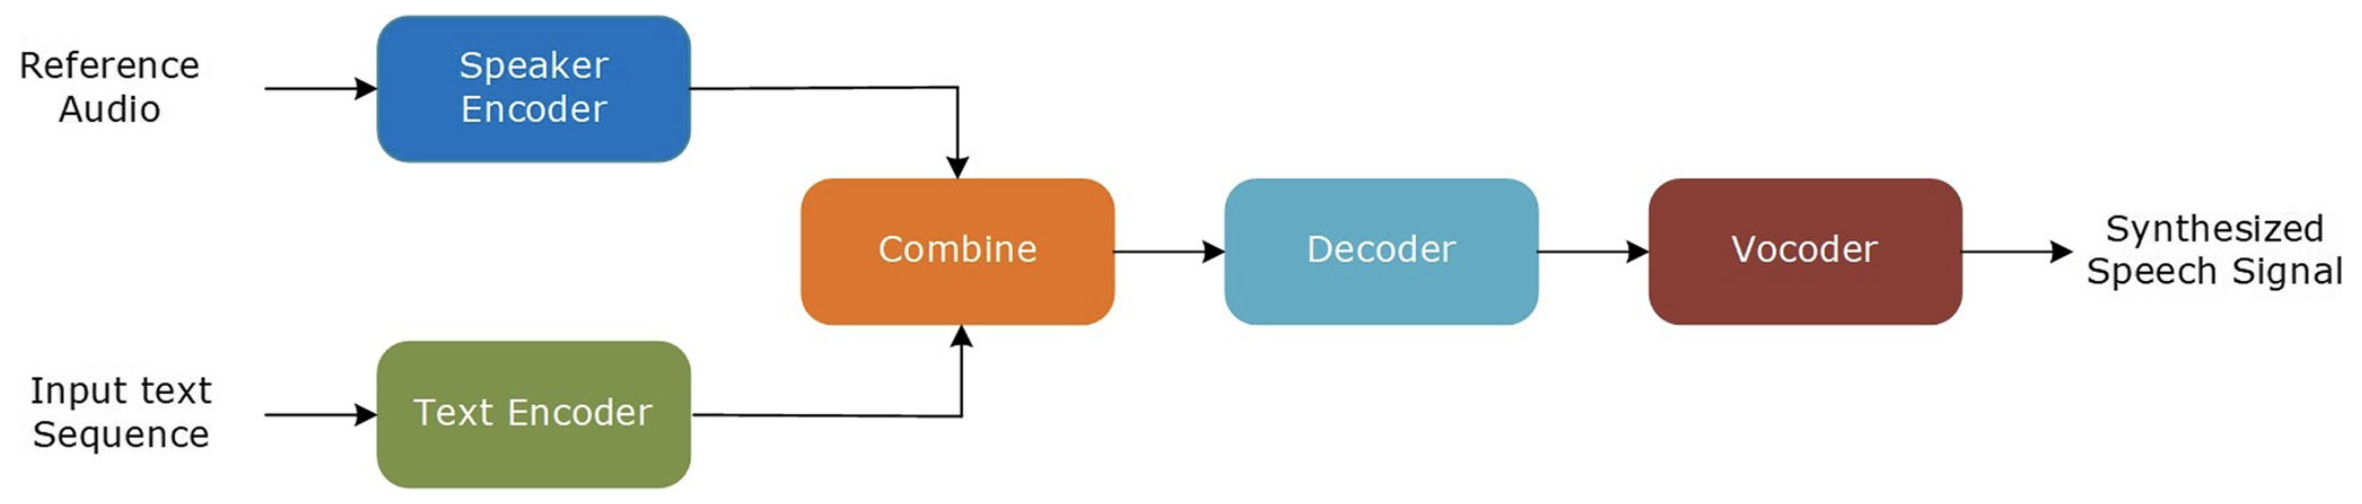
\includegraphics[width=0.95\textwidth]{assets/TTS.png}
  \caption[labelInTOC]{Workflow Diagramm der aktuellen TTS Systeme \citep[][]{Masood2022}}
  \label{fig:tts}
\end{center}
\end{figure}

Zunächst wird ein TTS Modell mithilfe von Audioaufnahmen sowie den dazugehörigen Transkripten auf eine Stimme trainiert.
Anschließend können Texte entgegengenommen, in zuvor gelernte Formen gebracht und so die Parameter für den letzten Schritt berechnet werden.
Mit diesen Parametern wird mittels Vocoder ein Audiosignal erzeugt, das dem gewünschten Text in einer möglichst menschenähnlichen Stimme entspricht.
Einige Beispiele für derartige Deeplearning Modelle sind WaveNet (2016), Tacotron2 (2018) und DeepVoice3 (2018) \citep[vgl.][]{Almutairi2022}.

Neueste Entwicklungen zeigen, dass dieser Prozess auch in Echtzeit möglich ist, wobei von Voice Cloning gesprochen wird.
Hierbei liegt der Fokus darauf, bestimmte Stimmfeatures zu erhalten wodurch nicht nur menschenähnliche Stimmen sondern gezielt Personen nachgeahmt werden können.
Diese Technologie ist frei zugängig, beispielsweise über Anwendungen wie Overdub oder VoiceApp und ermöglicht die Erstellung von AD \citep[][]{Masood2022}.

\textbf{Voice Conversion}\\
Eine andere Möglichkeit künstliche Sprachdateien zu erzeugen ist Voice Conversion.
Im Gegensatz zu TTS liegt als Eingabe eine Audiodatei vor, wobei die Stimme durch verschiedene Methoden so moduliert wird, dass die Ausgabe einer anderen Person zugeordnet werden kann.
Diese Modulierung basiert auf verschiedenen akustischen Features wie dem Stimmklang, der Betonung, Tempo und Sprechpausen.
Dementsprechend groß sind die Datenmengen, die benötigt werden um realistische Stimmen zu erzeugen.
Allerdings lassen sich so sehr gute Imitate erzeugen, zum Teil sogar in einer anderen Sprache, wenn die Qualität der zum Anlernen verwendeten Audiodaten entsprechen gut ist \citep[][]{Masood2022}.

Hier werden ähnlich wie bei TTS Vocoder verwendet, aber auch Neuronale Netze und Machine Learning mit speziellen Algorithmen zur Manipulation von multimedialen Inhalten.

Beide Technologien, sowohl TTS als auch VC, eignen sich prinzipiell für die Erzeugung von AD in Echtzeit beziehungsweise zur Verwendung in oben genannten Szenarien.
Voraussetzung ist jeweils, dass genug Material der Zielperson vorhanden ist, um die Modelle anzulernen.
\clearpage

\subsubsection{Audio Deepfake Detection}
Die zuvor vorgestellten Methoden zur künstlichen Stimmsynthese werden nicht nur für die Verbesserung von Mensch-Computer-Interaktionen verwendet, sondern auch zur Erzeugung von AD mit zum Teil kriminellen Absichten.
Um dem entgegenzuwirken wird intensiv an Algorithmen zur Erkennung von AD geforscht.

Grundsätzlich können die verfügbaren Methoden darin unterschieden werden, ob die zur Identifizierung von synthetischen Audiospuren verwendeten Features manuell oder per Deeplearning spezifiziert werden.
Andere Quellen sprechen auch von feature-based approach oder image-based approach \citep[][]{Khochare2021}.
Bis auf wenige Ausnahmen ist allen Methoden gemein, dass sie auf die Detektion bestimmter Generationsmechanismen (TTS oder VC) spezialisiert sind.
Dabei werden sie auf definierte Sammlungen von synthetisch erzeugten Audiodateien mit bekannten Erzeugungsmechanismen angelernt um anschließend Proben mit ähnlichen Features identifizieren zu können.

Beim feature-based approach werden die einzelnen Audiodateien manuell auf verschiedene spektrale Features untersucht und in einen entsprechenden Datensatz umgewandelt.
Dieser Datensatz wird mit einem Machine Learning Algorithmus verarbeitet um dem Algorithmus beizubringen, welche Features in den später zu untersuchenden Proben relevant sind.
Beim image-based approach wird das Audiosignal mittels Fast Fourier Transformation von der Zeit- in die Frequenzebene umgewandelt und anschließend die Amplitude in Dezibel konvertiert um ein Melspectrogram zu erhalten.
Mit verschiedenen Deep Learning Methoden werden anschließend die relevanten Features berechnet.

Für beide Varianten sind große Datenmengen, bestehend aus vielen oder langen Sequenzen, zum Anlernen erforderlich.
In der Literatur werden einige Datensätze genannt, mit denen Detektionsalgorithmen angelernt, aber auch getestet werden können.
So gibt es einen sehr großen open source Datensatz von Mozilla \citep[][]{Ardila2019}, mittlwerweile vier Datensätze aus den Jahren 2015, 2017, 2019 und 2021 von der ASVspoof Challenge\footnote{Automatic Speaker Verification Spoofing And Countermeasures Challenge, bei der es darum geht aktuelle Herausforderungen in der Erkennung von Audio Deepfakes zu bewältigen um die Sicherheit von ASV Systemen zu erhöhen\citep[][]{Yamagishi2021}} sowie weitere öffentlich zugängige Datensätze wie den fake-or-real (FOR) Datensatz \citep[][]{Reimao2019}. 
Dabei geht der Trend dahin, nicht mehr nur die grundsätzlichen Fähigkeiten von Detektionsalgorithmen zur Überprüfung von (Labor)Proben zu beweisen, sondern es werden vermehrt Audioproben erzeugt und getestet, die einen realen Angriff mit Fake Audio simulieren sollen.
Der FOR sowie der aktuellste Datensatz der ASVspoof Challenge enthalten Proben, die einen Angriff per Telefon oder Sprachnachricht simulieren sollen \citep[][]{Masood2022}.

Sind die Detektionsalgorithmen einmal angelernt können sie dazu verwendet werden, Audioproben zu testen um zu entscheiden, ob sie authentisch sind oder synthetisch erzeugt wurden.

Dabei gibt es jedoch einige Einschränkungen, die immer wieder in der Literatur genannt werden.
Folgende Tabelle gibt einen Überblick über die Herausforderungen, vor allem auch im Hinblick auf die Ausgangsfragestellung.
\clearpage

\begin{table}[htp]
\begin{center}
\begin{tabular}{L{10em}L{19em}L{8em}}
\multirow{2}{*}{\textbf{Herausforderung}} &\multirow{2}{*}{\textbf{Beschreibung}} &\textbf{Relevanz für Ausgangsfrage}\\
\toprule
\multirow{3}{*}{Anlernen} &Die Detektionsalgorithmen benötigen viele Daten zum Anlernen und hohe Rechenressourcen &\multirow{3}{*}{mittel}\\
\midrule
\multirow{3}{*}{Datenvorverarbeitung} &Audioproben müssen entweder aufwendig manuell aufbereitet oder mit hohem Rechenaufwand analysiert werden &\multirow{3}{*}{hoch}\\
\midrule
\multirow{3}{*}{Störgeräusche} &Außengeräusche wie Regen, Rauschen, Straßenlärm können die Detektion von AD verhindern &\multirow{3}{*}{hoch}\\
\midrule
\multirow{2}{*}{Sprache und Akzente} &Beschränkung der verfügbaren Trainingsdaten hauptsächlich auf Englisch &\multirow{2}{*}{mittel}\\
\midrule
\multirow{2}{*}{VC Detektion} &Im Gegensatz zu TTS werden mit VC erzeugte AD schlechter erkannt &\multirow{2}{*}{mittel}\\
\midrule
\multirow{3}{*}{Generalisierung} &Signifikant schlechtere Performance der Detektionsmethoden bei Proben mit anderem Erzeugungsmodell &\multirow{3}{*}{hoch}\\
\bottomrule
\end{tabular}
\caption{Einschränkungen und Herausforderungen aktueller AD Detektionsmethoden, zusammengestellt nach \citep[][]{Almutairi2022,Masood2022}}
\label{tab:challenge}
\end{center}
\end{table}

Das größte Problem, bezogen auf die Ausgangsfragestellung, ist der Prozess der Datenvorverarbeitung.
Für beide oben beschriebenen Varianten von Detektionsalgorithmen müssen zunächst relevante Features in den Proben  identifiziert werden.
Dazu wird entweder ein Data Scientist benötigt, der diese manuell ermittelt (hoher Zeitaufwand), oder hohe Rechenressourcen um den Prozess über Deep Learning zu automatisieren.

Wie bereits zu Beginn des Abschnitts erwähnt, sind die verfügbaren AD Methoden grundsätzlich auf die Erkennung eines Erzeugungsmodells spezialisiert.
Viele Methoden sind dabei auf die Erkennung von TTS ausgerichtet.
Besonders realistische Imitate lassen sich jedoch mit VC erreichen, wobei die Erkennung laut M. Ballesteros et al. \glqq{}nicht trivial\grqq{} ist \citep[][]{Ballesteros2021}.

Weitere Einschränkungen sind Störgeräusche oder eine Zusammensetzung von authentischen und synthetischen Teilen in den Audioproben.
Dies führt bei vielen entwickelten AD Methoden zu deutlich schlechteren Erkennungsraten oder einem erheblich höheren Rechenaufwand \citep[][]{Masood2022}.

Bei den Literaturübersichten von Masood et al. und Almutairi et al. ist zu erkennen, dass bei den aktuell verfügbaren Detektionsalgorithmen in der Regel ein bis zwei der in Tabelle~\ref{tab:challenge} aufgeführten Herausforderungen gut gelöst werden.
Allerdings bringt das auch immer Limitationen mit sich.
Wenn beispielsweise ein Algorithmus robust gegen Störgeräusche ist, dann geht das mit einem stark erhöhten Rechenaufwand einher.
Können TTS Proben gut erkannt werden, dann werden VC Proben nicht erkannt.
Ist die Genauigkeit der Detektion sehr gut, werden große Mengen an Trainingsdaten benötigt \citep[][]{Masood2022,Almutairi2022}.

Eine allgemeingültige Lösung für die Detektion von Audio Deepfakes in Alltagssituationen, besonders die zeitkritische Analyse von Proben mit Störgeräuschen gibt es bislang nicht.
Allerdings rückt die Analyse von \glqq{}real world samples\grqq{} immer mehr in den Fokus der Wissenschaft und wird auch im Rahmen der ASVspoof Challenges immer wichtiger \citep[][]{Yamagishi2021,Liu2022}.

%\subsection{Effektivität und Effizienz}
% Fokus auf Echtzeitproblematik: Was ist technisch möglich oder eben nicht?
% Hier erstes kleines Fazit ziehen?
\subsection{Fast Detection}
\begin{itemize}
  \item ganz aktueller, interessanter Ansatz \citep[][]{Kawa2022}
  \item bewusst auf state-of-the-art Genauigkeit verzichten
  \item dadurch Rechenleistung einsparen $\rightarrow$ Detection quasi auf jedem Gerät möglich
  \item Annahme: nicht jeder Fake ist super durchorganisiert mit modernstem Equipment (wie bereits gezeigt kann jeder mit seinem Handy etc. einen ordentlichen Fake herstellen) $\rightarrow$ automatisierte Detektion, auch große batch size möglich
  \item $\rightarrow$ parallele zu Malware: sehr gute richtet Schaden an und ist schwer zu detektieren, aber der größte Teil kann durch \glqq{}einfache\grqq{} Vorsichtsmaßnahmen bzw. Software verhindert werden
\end{itemize}